\documentclass[conference]{IEEEtran}
\IEEEoverridecommandlockouts

% ---------- Packages ----------
\usepackage{cite}
\usepackage{amsmath,amssymb,amsfonts}
\usepackage{graphicx}
\usepackage{booktabs}
\usepackage{multirow}
\usepackage{textcomp}
\usepackage{xcolor}
\usepackage{url}
\usepackage{tikz}
\usetikzlibrary{positioning,arrows.meta,fit}

% Placeholders for content that depends on the final experiments.
% Every \TODO must be resolved (or removed) before submission.
\newcommand{\TODO}[1]{\textcolor{red}{\textbf{[TODO: #1]}}}

\begin{document}

\title{ENSO-Aware Adversarial Forecasting: A Unified WGAN-GP Framework for Extreme-Aware Imputation and Forecasting of Heatwave Days in Regional Temperature Time Series}

% ---------- Authors ----------
% TODO: confirm author order, add e-mail addresses, and follow the VIT Chennai
% authorship policy.
\author{
\IEEEauthorblockN{Melvin Immanuel G}
\IEEEauthorblockA{\textit{Department of Mathematics} \\
\textit{School of Advanced Sciences} \\
\textit{Vellore Institute of Technology}\\
Chennai, India}
\and
\IEEEauthorblockN{Nainor Selvan G}
\IEEEauthorblockA{\textit{Department of Mathematics} \\
\textit{School of Advanced Sciences} \\
\textit{Vellore Institute of Technology}\\
Chennai, India}
\and
\IEEEauthorblockN{Prof.\ Dr.\ Kalyani Desikan}
\IEEEauthorblockA{\textit{Department of Mathematics} \\
\textit{School of Advanced Sciences} \\
\textit{Vellore Institute of Technology}\\
Chennai, India}
}

\maketitle

\begin{abstract}
Weather and climate time series are simultaneously non-stationary, gap-prone, and characterized by
rare but high-impact extreme events such as heatwaves. Over India, the frequency and persistence of
heatwaves are further modulated by the El Ni\~{n}o--Southern Oscillation (ENSO), so that the days of
greatest practical consequence cluster in El Ni\~{n}o-affected seasons. Existing generative adversarial
network (GAN) approaches to this domain address imputation and forecasting as separate problems, ignore
large-scale climate drivers such as ENSO, and existing extreme-value-aware adversarial objectives have
been demonstrated on financial series or on continental-scale spatial climate fields rather than on
region- or city-scale time series. We propose a unified adversarial framework in which a single
ENSO-conditioned generator performs both missing-data imputation and multi-step forecasting of heatwave
days for a regional temperature series, trained with a Wasserstein GAN with gradient penalty (WGAN-GP)
objective augmented by a generalized-extreme-value-inspired exceedance-weighted loss term. The generator
and critic are conditioned on a causally lagged Oceanic Ni\~{n}o Index, so that the model can learn how
the likelihood and intensity of heatwave days shift with the ENSO phase. The framework is evaluated under
a temporally held-out train/validation/test protocol using both continuous-value metrics (RMSE, MAE,
R\textsuperscript{2}, extreme-tail RMSE) and event-level detection metrics (probability of detection,
false alarm ratio, critical success index) aligned to the India Meteorological Department heatwave
definition, reported separately for El Ni\~{n}o, La Ni\~{n}a and neutral periods, enabling direct
comparison with classification-based heatwave studies. \TODO{Replace with a 2--3 sentence summary of the
final quantitative results once real-data experiments are complete, e.g.\ ``On $N$ years of ERA5-Land
data for Chennai, the proposed framework improves heatwave-event CSI by X\% over the strongest classical
baseline during El Ni\~{n}o periods while remaining competitive on bulk RMSE.''}
\end{abstract}

\begin{IEEEkeywords}
generative adversarial networks, WGAN-GP, time series imputation, weather forecasting, extreme value
theory, heatwave prediction, El Ni\~{n}o--Southern Oscillation, ERA5-Land
\end{IEEEkeywords}

% =====================================================================
\section{Introduction}
\label{sec:intro}

Missing observations and the need to project future states are two persistent, related challenges in
regional climate time series analysis. Sensor outages, transmission loss, and irregular station
coverage all produce gaps that must be filled before a series can be analyzed or modeled, while
downstream applications such as early-warning systems require genuine forecasts of future values. Both
problems are compounded when the quantity of interest is prone to extreme excursions: temperature
time series in tropical, heatwave-prone regions such as peninsular India are dominated in aggregate by
smooth seasonal and diurnal cycles, yet the events of greatest practical consequence---heatwaves---sit
in the tail of the distribution, precisely where models trained under a mean-squared-error
objective are known to be least reliable.

\TODO{Expand this paragraph with 1--2 sentences on the human/economic impact of heatwaves in India
specifically (cite a recent IMD or health-impact source), to motivate the practical stakes before
moving to the technical gap.}

Heatwave occurrence over India is not stationary from year to year. The El Ni\~{n}o--Southern
Oscillation (ENSO), the dominant mode of interannual climate variability in the tropical Pacific
\cite{trenberth1997definition,mcphaden2006enso}, influences Indian surface temperature through
atmospheric teleconnections, and the frequency and duration of Indian heatwaves have been linked to
warm (El Ni\~{n}o) conditions in the central and eastern Pacific
\cite{rohini2016variability,ratnam2016anatomy}. This relationship is itself non-stationary
\cite{kumar1999weakening}, which makes it a natural candidate for data-driven rather than fixed
parametric modeling. A model that imputes or forecasts temperature without access to the ENSO state
must treat El Ni\~{n}o and La Ni\~{n}a years as draws from a single distribution, and is therefore
likely to under-predict exactly the heatwave days that cluster in El Ni\~{n}o-affected seasons.

Generative adversarial networks (GANs) \cite{goodfellow2014generative} have been applied productively
to both imputation \cite{luo2018multivariate,zhao2024qar} and forecasting/generation
\cite{bihlo2021generative,balogun2024temperaturegan,glawion2025spateganera5} of weather and climate
data, and a separate line of work has shown that explicitly reshaping the training objective around
extreme value theory (EVT) improves tail fidelity in both non-adversarial
\cite{ding2019modeling,zhang2021enhancing} and adversarial
\cite{huster2021pareto,bhatia2021exgan,boulaguiem2022modeling,liu2025deepxgan} settings. As detailed
in Section~\ref{sec:related}, however, no existing framework combines imputation and forecasting within
a single adversarially-trained generator for a region-scale series, no extreme-value-aware GAN has been
applied to city- or region-scale temperature imputation/forecasting in a heatwave-prone setting such as
India, and none conditions on the ENSO state that modulates heatwave risk. A recent, closely related
study on Chennai heatwave classification \cite{choudary2025comparative} explicitly names time series
GANs as a plausible, unexplored strategy for handling the class imbalance inherent to rare heatwave
events, but does not pursue it.

This paper makes the following contributions:
\begin{enumerate}
    \item A unified adversarial framework in which a single generator performs both interior-gap
    imputation and multi-step forecasting, differing only in where the reconstruction mask falls within
    a training window.
    \item ENSO conditioning of both the generator and the WGAN-GP critic on a causally lagged Oceanic
    Ni\~{n}o Index (ONI), so that imputed and forecast heatwave days are generated conditionally on the
    El Ni\~{n}o, La Ni\~{n}a or neutral state of the tropical Pacific.
    \item A generalized-extreme-value-inspired exceedance-weighted loss term that makes the
    reconstruction objective explicitly sensitive to tail (heatwave) behavior, combined with a WGAN-GP
    adversarial objective \cite{arjovsky2017wasserstein,gulrajani2017improved}.
    \item A rigorous, temporally held-out evaluation protocol---avoiding a data-leakage failure mode we
    identified in early iterations of this work (Section~\ref{sec:methods})---reporting both continuous
    and event-level (POD/FAR/CSI) metrics, stratified by ENSO phase, for direct comparability with
    classification-style heatwave studies.
    \item \TODO{An empirical evaluation on \_\_ years of ERA5-Land data for \_\_ (city/region), showing
    \_\_.}
\end{enumerate}

% =====================================================================
\section{Related Work}
\label{sec:related}

\subsection{Statistical and Deep Learning Approaches to Weather Time Series}

Classical statistical models such as ARIMA and SARIMA remain common baselines for climate time series
owing to their interpretability and modest data requirements, but they assume linear, stationary
dynamics and struggle with the non-linear, non-stationary behavior typical of real weather data
\cite{alejosanchez2025missing}. Recurrent architectures such as LSTM and hybrid CNN-LSTM networks
capture non-linear temporal dependencies directly from data, but models trained under a
mean-squared-error objective regress toward the conditional mean, systematically under-representing
tail events such as heatwaves \cite{alejosanchez2025missing}. This smoothness bias motivates the shift
toward generative and distribution-aware modeling reviewed below.

\subsection{Generative Adversarial Approaches to Climate and Weather Data}

GANs have been applied to weather and climate data along two largely separate tracks: imputation, and
generation/forecasting. On the imputation side, Luo et al.~\cite{luo2018multivariate} introduced an
early GAN-based framework for multivariate time series imputation, and Zhao et al.~\cite{zhao2024qar}
added a self-attention discriminator for imputing aviation time series; neither targets
weather-specific tail behavior, and both evaluate imputation in isolation from any downstream
forecasting task. On the generation/forecasting side, Bihlo~\cite{bihlo2021generative} trained a
conditional deep convolutional GAN on ERA5 reanalysis to forecast 24-hour-ahead geopotential height,
2\,m temperature, and precipitation over Europe; Balogun et al.~\cite{balogun2024temperaturegan}
instead perform unconditional stochastic generation of hourly 2\,m temperature fields conditioned on
month, region, and time-of-day; and Glawion et al.~\cite{glawion2025spateganera5} downscale ERA5
precipitation to kilometer and sub-hourly resolution with explicit evaluation of extreme rainfall
preservation. Across this body of work, imputation and forecasting are treated as separate problems
solved by separately trained generators, conditioning is limited to calendar or regional information
rather than large-scale climate drivers such as ENSO, and none are evaluated on India or on
heatwave-prone tropical climates.

\subsection{Extreme-Value-Aware and Tail-Focused Generative Modeling}

A parallel line of research reshapes the training objective around the tail of the distribution rather
than its mean. Ding et al.~\cite{ding2019modeling} proposed an extreme value loss for time series
prediction that reweights the objective using a fitted extreme value distribution, later generalized by
Zhang et al.~\cite{zhang2021enhancing}. Within GAN architectures, the Pareto-GAN of Huster et
al.~\cite{huster2021pareto} extends generator representational capacity into heavy-tailed regimes
using extreme value theory, and the ExGAN of Bhatia et al.~\cite{bhatia2021exgan} conditions sample
generation directly on user-specified extremeness. Boulaguiem et al.~\cite{boulaguiem2022modeling}
combine EVT with a GAN discriminator for spatial extremes, and the most climate-specific recent
example, the DeepX-GAN of Liu et al.~\cite{liu2025deepxgan}, embeds a spatial extremal-dependence
metric into the discriminator to generate physically plausible unseen heat extremes across the Middle
East and North Africa. This family of work establishes that tail-aware adversarial objectives
measurably outperform vanilla adversarial or MSE-only training on extreme-event fidelity---but every
example operates on financial data, generates unconditional spatial fields, or targets
continental-scale spatial extremes, rather than gap-filling and forecasting a specific city-scale time
series.

\subsection{Heatwave-Specific Prediction, with Emphasis on India}

Jacques-Dumas et al.~\cite{jacquesdumas2022deep} trained a CNN on climate-model output with
class-undersampling and transfer learning to forecast long-lasting heatwaves, addressing the severe
class imbalance inherent to rare-event prediction. Alhusainan et al.~\cite{alhusainan2025forecasting}
combined ConvLSTM, transformer-based temporal attention, and physics-informed constraints to forecast
extreme heat in Kuwait from hourly ERA5-Land data, using ARIMA/SARIMA as classical baselines---a design
closely related in spirit, though not architecture, to the present work. Within India specifically,
Ratnam et al.~\cite{ratnam2023predicting} used machine learning to predict maximum temperatures ten days
ahead, and---most directly relevant---Choudary et al.~\cite{choudary2025comparative} benchmarked nine
machine learning classifiers for next-day heatwave event classification on fourteen years of Chennai
(Tambaram) station data, reporting a best accuracy of 98.92\% with a CNN. Qureshi et
al.~\cite{qureshi2025developing} developed a seasonal-adjusted hybrid time series model for heatwave
warning under a similar rare-event framing. Notably, Choudary et al.~\cite{choudary2025comparative}
explicitly identify time series GANs as a plausible strategy for generating temporally coherent
synthetic minority-class sequences to address class imbalance, but do not implement or evaluate the
approach, leaving it as an open direction that this work pursues.

\subsection{ENSO and Indian Heatwaves}

ENSO is conventionally monitored through sea surface temperature (SST) anomalies in the Ni\~{n}o-3.4
region \cite{trenberth1997definition}; the NOAA Oceanic Ni\~{n}o Index (ONI), a three-month running
mean of ERSSTv5 Ni\~{n}o-3.4 anomalies \cite{huang2017ersstv5,noaa_oni}, defines El Ni\~{n}o (La
Ni\~{n}a) episodes as periods in which the ONI is at or above $+0.5\,^{\circ}$C (at or below
$-0.5\,^{\circ}$C) for at least five consecutive overlapping seasons. Rohini et al.~\cite{rohini2016variability}
showed that heatwave frequency and duration over India have increased and are associated with
positive SST anomalies in the central and eastern Pacific, and Ratnam et al.~\cite{ratnam2016anatomy}
related Indian heatwaves to large-scale circulation anomalies forced from the tropical oceans. The
ENSO--Indian climate link has also weakened and strengthened over recent decades
\cite{kumar1999weakening}. Despite this physical motivation, the data-driven heatwave studies reviewed
above do not use the ENSO state as a model input, and none evaluate skill separately in El Ni\~{n}o
and La Ni\~{n}a years.

\subsection{Research Gap}

Four gaps emerge from this survey. First, GAN-based imputation and GAN-based forecasting/generation
have developed as separate literatures; no framework performs both within a single
adversarially-trained generator for the same regional dataset. Second, extreme-value-aware adversarial
objectives have been demonstrated on financial series or on continental/global spatial climate fields,
but not on a city- or region-scale time series task that combines imputation and forecasting. Third,
the most directly comparable India-focused study explicitly flags time series GAN generation as an
unexplored strategy for heatwave-related class imbalance, without pursuing it
\cite{choudary2025comparative}. Fourth, although ENSO is a documented driver of Indian heatwave
variability \cite{rohini2016variability,ratnam2016anatomy}, no generative imputation or forecasting
model for Indian temperature conditions on the ENSO state or reports its skill by ENSO phase. This work
addresses all four.

% =====================================================================
\section{Data}
\label{sec:data}

\TODO{Fill in final data description once the full pull is complete. Draft below based on the
Review-1 pipeline, extended per the revised scope.}

\subsection{Regional Temperature Series}

Daily meteorological data were obtained from the ERA5-Land reanalysis product
\cite{munozsabater2021era5land,hersbach2020era5} (\texttt{ECMWF/ERA5\_LAND/DAILY\_AGGR}) via the Google
Earth Engine API \cite{gorelick2017gee}, for a point located at \TODO{13.08\,\textdegree N,
80.23\,\textdegree E (Chennai)} / \TODO{list any additional cities if the multi-site extension is
pursued}, covering \TODO{2010-01-01 to 2024-12-31 (15 years). Note: the ENSO-stratified evaluation needs
several El Ni\~{n}o and La Ni\~{n}a episodes in each of the training and test periods; the 1950--2025
extract already in the project repository is better suited to this than a 15-year window.}. Variables
extracted include 2\,m air temperature (\texttt{temperature\_2m}), surface pressure, total
precipitation, and \TODO{any additional variables: dewpoint temperature, wind components, etc.}.
\TODO{Because the IMD heatwave definition is stated in terms of daily maximum temperature, also extract
\texttt{temperature\_2m\_max} and use it as the heatwave target.} Temperature values were converted from
Kelvin to Celsius. The series was split chronologically into training (\TODO{2010--2020}), validation
(\TODO{2021--2022}), and test (\TODO{2023--2024}) partitions, with all scaling parameters and
extreme-value thresholds fit on the training partition only to avoid information leakage from
validation/test periods into model development.

\subsection{ENSO Index}

The ENSO state is represented by the monthly ONI \cite{noaa_oni}, computed from ERSSTv5 Ni\~{n}o-3.4
SST anomalies \cite{huang2017ersstv5}. Each calendar month is labeled El Ni\~{n}o, La Ni\~{n}a, or
neutral using the NOAA episode rule given in Section~\ref{sec:related}, and the monthly ONI is mapped
to daily resolution by assigning each day the value of its month. Because the ONI is a centered
three-month mean, the value for a given month uses SST from the following month; to keep the
forecasting task operationally causal, the conditioning variable for a window starting on day $t_0$ is
the most recent ONI value that would have been published before $t_0$, i.e., the ONI lagged by
$\ell \geq 2$ months. \TODO{Report the number of El Ni\~{n}o, La Ni\~{n}a and neutral months in the
training, validation and test partitions.}

\subsection{Heatwave Days}

Heatwave days are labeled following the India Meteorological Department (IMD) criteria
\cite{imd2024heatwave}. For a coastal station such as Chennai, a heatwave may be declared when the
daily maximum temperature departs from its calendar-day climatological normal by at least
$4.5\,^{\circ}$C and the actual maximum temperature is at least $37\,^{\circ}$C; a departure of more
than $6.4\,^{\circ}$C denotes a severe heatwave. Calendar-day normals are computed from the training
partition only. \TODO{ERA5-Land is a gridded reanalysis and may be biased relative to station maxima;
state whether the absolute $37\,^{\circ}$C condition is kept, bias-corrected against IMD station data,
or replaced by a training-period percentile threshold, and report the resulting number of heatwave days
per partition and per ENSO phase.}

% =====================================================================
\section{Methods}
\label{sec:methods}

\begin{figure}[t]
\centering
\resizebox{\columnwidth}{!}{% Framework diagram shared by main.tex and snippet.tex (requires tikz with
% the positioning, arrows.meta and fit libraries).
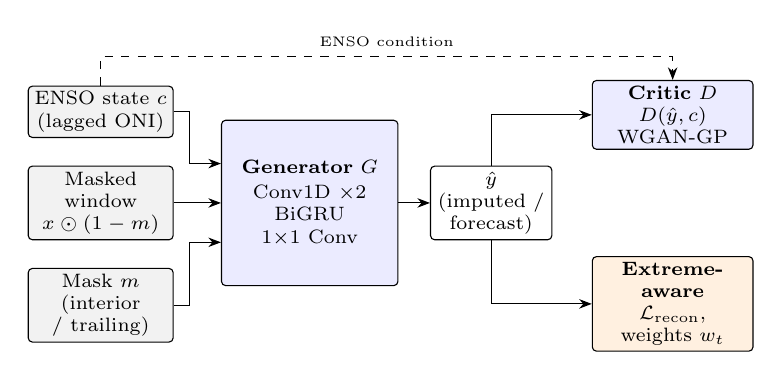
\begin{tikzpicture}[
  font=\scriptsize,
  >={Stealth[length=1.6mm]},
  node distance=3.5mm and 4mm,
  box/.style={draw, rounded corners=1.5pt, align=center, minimum height=6.5mm, inner sep=2pt, fill=white},
  inp/.style={box, fill=gray!10, text width=17mm},
  net/.style={box, fill=blue!8, text width=19mm},
  loss/.style={box, fill=orange!12, text width=19mm}
]
  % Inputs
  \node[inp] (c)   {ENSO state $c$\\(lagged ONI)};
  \node[inp, below=of c] (x)   {Masked window\\$x \odot (1-m)$};
  \node[inp, below=of x] (m)   {Mask $m$\\(interior / trailing)};

  % Generator
  \node[net, right=6mm of x, text width=21mm, minimum height=21mm] (G)
    {\textbf{Generator $G$}\\[1pt] Conv1D $\times 2$\\ BiGRU\\ $1{\times}1$ Conv};

  % Output
  \node[box, right=of G, text width=14mm] (yhat) {$\hat{y}$\\(imputed /\\forecast)};

  % Critic and loss
  \node[net, above right=2mm and 5mm of yhat] (D) {\textbf{Critic $D$}\\$D(\hat{y}, c)$\\WGAN-GP};
  \node[loss, below right=2mm and 5mm of yhat] (L) {\textbf{Extreme-aware}\\$\mathcal{L}_{\mathrm{recon}}$, weights $w_t$};

  % Arrows
  \draw[->] (c.east) -- ++(2mm,0) |- ([yshift=5mm]G.west);
  \draw[->] (x.east) -- (G.west);
  \draw[->] (m.east) -- ++(2mm,0) |- ([yshift=-5mm]G.west);
  \draw[->] (G) -- (yhat);
  \draw[->] (yhat.north) |- (D.west);
  \draw[->] (yhat.south) |- (L.west);
  \coordinate (top) at ([yshift=3mm]D.north);
  \draw[->, dashed] (c.north) |- node[pos=0.75, above, font=\tiny] {ENSO condition} (top) -- (D.north);
\end{tikzpicture}
}
\caption{Proposed ENSO-aware framework. A single generator receives a masked temperature window, the
mask, and the lagged ENSO state, and fills either an interior gap (imputation) or the trailing $k$ days
(forecasting). It is trained with an ENSO-conditioned WGAN-GP critic and an extreme-aware weighted
reconstruction loss.}
\label{fig:framework}
\end{figure}

\subsection{Problem Formulation}

We formulate imputation and forecasting as a single masked-reconstruction problem. Given a window of
length $W$ drawn from the scaled temperature series, a binary mask $m \in \{0,1\}^W$ indicates which
positions are hidden from the model. When the masked span sits in the interior of the window, the task
is imputation; when the masked span is the trailing $k$ steps of the window with no observations beyond
it, the task is equivalent to a $k$-step-ahead forecast. During training, the mask type (interior vs.\
trailing), position, and length are resampled independently for every window, which is the key
methodological safeguard against the failure mode we identified in early development of this project:
in an earlier iteration, a single fixed masked block was used for both training and evaluation, so the
generator was directly supervised, over hundreds of training epochs, to reconstruct the exact segment it
was later scored on, while classical baselines (ARIMA, SARIMA, KNN) never had access to it. This produced
implausible results (generator R\textsuperscript{2} $\approx$ 0.99 against negative-R\textsuperscript{2}
classical baselines) that we do not consider valid and have discarded in favor of the protocol described
here.

Each window is accompanied by a conditioning vector $c \in \mathbb{R}^{W \times d_c}$ that carries the
lagged ONI described in Section~\ref{sec:data} and, optionally, a sine--cosine encoding of the day of
the year. The generator therefore learns the conditional distribution
$p(y_{\mathcal{M}} \mid y_{\bar{\mathcal{M}}}, c)$ of the hidden values $y_{\mathcal{M}}$ given the
observed context $y_{\bar{\mathcal{M}}}$ and the ENSO state, rather than a single distribution pooled
over all ENSO phases.

\subsection{Generator and Critic Architecture}

The generator is a shared backbone consisting of two 1-D convolutional layers (kernel size 5) over the
input channels (masked value, mask indicator, and the ENSO conditioning channels $c$), followed by a
bidirectional GRU and a final $1\times1$ convolution projecting back to a single output channel. The
same generator, without architectural modification, is used for both imputation and forecasting
windows.

The critic follows the Wasserstein GAN with gradient penalty (WGAN-GP) formulation
\cite{arjovsky2017wasserstein,gulrajani2017improved}: a convolutional critic outputs an unbounded
realism score rather than a bounded probability, and a gradient penalty term enforces the Lipschitz
constraint required for the Wasserstein distance approximation to be meaningful. Following the
conditional GAN formulation \cite{mirza2014conditional}, the critic receives the conditioning channels
$c$ concatenated with the completed window, so that it judges whether a heatwave sequence is realistic
\emph{for the given ENSO state}. The critic loss is
\begin{equation}
\mathcal{L}_D = \mathbb{E}\big[D(\hat{x}, c)\big] - \mathbb{E}\big[D(x, c)\big]
+ \gamma\, \mathbb{E}\Big[\big(\lVert \nabla_{\tilde{x}} D(\tilde{x}, c) \rVert_2 - 1\big)^2\Big],
\label{eq:critic}
\end{equation}
where $x$ is a real window, $\hat{x}$ the generator-completed window, $\tilde{x}$ a random
interpolation between the two, and $\gamma$ the gradient-penalty weight. This was a deliberate design
choice over the vanilla discriminator used in early iterations of this work, where the adversarial loss
term was weighted more than three orders of magnitude below the reconstruction loss term and therefore
contributed negligibly to training---in that configuration the model was, in substance, a supervised
reconstruction network rather than a GAN.

\subsection{Extreme-Value-Aware Loss}

To make the reconstruction objective sensitive to tail behavior, we introduce an exceedance-weighted
mean-squared-error term inspired by the extreme value loss of Ding et al.~\cite{ding2019modeling} and
its generalization by Zhang et al.~\cite{zhang2021enhancing}. Let $\tau_t$ denote an extreme-value
threshold for day $t$ (e.g., the 95th percentile of the training distribution, or the IMD heatwave
threshold of Section~\ref{sec:data}, i.e., the calendar-day normal plus $4.5\,^{\circ}$C), and $\sigma$
the training standard deviation. For a true value $y_t$ and generator output $\hat y_t$ at masked
position $t$, we define a per-timestep weight
\begin{equation}
w_t = 1 + \lambda \cdot \max\!\left(0, \frac{y_t - \tau_t}{\sigma}\right),
\label{eq:weight}
\end{equation}
and the reconstruction loss is the $w_t$-weighted mean squared error over masked positions,
\begin{equation}
\mathcal{L}_{\text{recon}} = \frac{1}{|\mathcal{M}|}\sum_{t \in \mathcal{M}} w_t (\hat y_t - y_t)^2,
\label{eq:recon}
\end{equation}
where $\mathcal{M}$ is the set of masked positions in a batch and $\lambda$ controls the strength of the
extreme-event emphasis. This is a deliberately simplified, differentiable approximation of the full
GEV-likelihood-based reweighting in \cite{ding2019modeling} and \cite{zhang2021enhancing}; we describe
it here as an adaptation rather than a reproduction, and note that fitting a full generalized Pareto or
GEV distribution to the residual exceedances is a natural extension for future work
(Section~\ref{sec:discussion}).

The full generator objective combines the adversarial term with this weighted reconstruction term:
\begin{equation}
\mathcal{L}_G = -\mathbb{E}\big[D(\hat{x}, c)\big] + \beta \, \mathcal{L}_{\text{recon}},
\label{eq:gen}
\end{equation}
with $\beta$ chosen so that the adversarial and reconstruction terms are of comparable magnitude
(\TODO{report final $\beta$, $\lambda$, $\gamma$ values used}).

\subsection{ENSO-Balanced Training}

El Ni\~{n}o months are a minority of the record, and heatwave days are a minority within them. To keep
the generator from fitting mainly the neutral-phase climatology, training windows are drawn with
probabilities that equalize the three ENSO phases within each mini-batch, while validation and test
windows are left at their natural frequencies. \TODO{Confirm whether phase-balanced sampling is used in
the final runs, and report its effect in the ablation table.}

\subsection{Baselines and Ablations}

ARIMA, SARIMA, and $k$-nearest-neighbor (KNN) baselines are fit per window using only the observed
(non-masked) context---for interior gaps, the pre- and (where applicable) post-gap context; for
trailing (forecast) gaps, only the pre-gap context, exactly matching the information a deployed
forecasting system would have. All baselines are scored on the identical held-out windows as the
proposed model. We additionally report the following ablations, each retaining the generator
architecture:
\begin{itemize}
    \item \emph{No adversarial term} ($\beta \to \infty$ equivalent, i.e.\ reconstruction loss only, no
    critic), to isolate the marginal contribution of the adversarial objective itself;
    \item \emph{No ENSO conditioning}, in which $c$ is removed from both the generator and the critic;
    \item \emph{Shuffled ENSO}, in which the ONI series is permuted across years, as a control showing
    whether any gain comes from the ENSO signal itself rather than from the extra input channel;
    \item \emph{ONI lag}, varying $\ell \in \{2, 3, 6\}$ months, to measure how far ahead the ENSO state
    carries useful information about heatwave days.
\end{itemize}
\TODO{Add LSTM baseline results if included in the final comparison.}

\subsection{Evaluation Protocol}

We report continuous-value metrics---RMSE, MAE, R\textsuperscript{2}, and an extreme-subset RMSE
restricted to true values exceeding $\tau_t$---alongside event-level detection metrics standard in
operational meteorological verification: probability of detection
($\text{POD} = TP/(TP+FN)$), false alarm ratio ($\text{FAR} = FP/(TP+FP)$), and critical success index
($\text{CSI} = TP/(TP+FP+FN)$), where an ``event'' is a masked day that meets the heatwave criterion of
Section~\ref{sec:data}. Where possible, $\tau_t$ is aligned with the India Meteorological Department's
operational heatwave definition (departure from the calendar-day climatological normal, rather than a
fixed percentile) once sufficient years of data are available to compute reliable normals. All metrics
are reported over the full test period and separately for El Ni\~{n}o, La Ni\~{n}a, and neutral months,
since a model may improve heatwave detection in El Ni\~{n}o periods while leaving its aggregate score
almost unchanged. Differences in forecast error between the proposed model and each baseline are tested
with the Diebold--Mariano test \cite{diebold1995comparing}. This choice of metrics allows direct
comparison with classification-based heatwave studies such as \cite{choudary2025comparative} and
\cite{qureshi2025developing}, which report precision/recall-style scores rather than continuous error.

% =====================================================================
\section{Results}
\label{sec:results}

\TODO{This entire section is a template pending real-data experiments. Replace
Tables~\ref{tab:results}--\ref{tab:ablation} with the actual test-set numbers, run across multiple
random seeds, and report mean $\pm$ std. Do not submit placeholder numbers---the tables only show the
expected format and are explicitly not experimental results.}

\begin{table*}[t]
\centering
\caption{Test-set results over the full test period (mean $\pm$ std over $\geq 3$ seeds). Populate with
real ERA5-Land test-set numbers.}
\label{tab:results}
\begin{tabular}{lccccccc}
\toprule
Model & RMSE & MAE & R\textsuperscript{2} & Extreme RMSE & POD & FAR & CSI \\
\midrule
Proposed (ENSO-cond.\ WGAN-GP + EVT loss) & \TODO{} & \TODO{} & \TODO{} & \TODO{} & \TODO{} & \TODO{} & \TODO{} \\
Ablation (no adversarial term) & \TODO{} & \TODO{} & \TODO{} & \TODO{} & \TODO{} & \TODO{} & \TODO{} \\
Ablation (no ENSO conditioning) & \TODO{} & \TODO{} & \TODO{} & \TODO{} & \TODO{} & \TODO{} & \TODO{} \\
ARIMA & \TODO{} & \TODO{} & \TODO{} & \TODO{} & \TODO{} & \TODO{} & \TODO{} \\
SARIMA & \TODO{} & \TODO{} & \TODO{} & \TODO{} & \TODO{} & \TODO{} & \TODO{} \\
KNN & \TODO{} & \TODO{} & \TODO{} & \TODO{} & \TODO{} & \TODO{} & \TODO{} \\
\bottomrule
\end{tabular}
\end{table*}

\begin{table}[t]
\centering
\caption{Heatwave-day detection by ENSO phase on the test period (CSI, mean $\pm$ std over $\geq 3$
seeds).}
\label{tab:enso}
\resizebox{\columnwidth}{!}{%
\begin{tabular}{lccc}
\toprule
Model & El Ni\~{n}o & Neutral & La Ni\~{n}a \\
\midrule
Proposed & \TODO{} & \TODO{} & \TODO{} \\
No ENSO conditioning & \TODO{} & \TODO{} & \TODO{} \\
Shuffled ENSO & \TODO{} & \TODO{} & \TODO{} \\
Strongest classical baseline & \TODO{} & \TODO{} & \TODO{} \\
\midrule
Heatwave days in test period & \TODO{} & \TODO{} & \TODO{} \\
\bottomrule
\end{tabular}%
}
\end{table}

\begin{table}[t]
\centering
\caption{Ablation over the ONI lag $\ell$ and the extreme-loss strength $\lambda$ (test period).}
\label{tab:ablation}
\resizebox{\columnwidth}{!}{%
\begin{tabular}{lcccc}
\toprule
Setting & RMSE & Extreme RMSE & POD & CSI \\
\midrule
$\ell = 2$ months & \TODO{} & \TODO{} & \TODO{} & \TODO{} \\
$\ell = 3$ months & \TODO{} & \TODO{} & \TODO{} & \TODO{} \\
$\ell = 6$ months & \TODO{} & \TODO{} & \TODO{} & \TODO{} \\
\midrule
$\lambda = 0$ (plain MSE) & \TODO{} & \TODO{} & \TODO{} & \TODO{} \\
$\lambda = $ \TODO{} & \TODO{} & \TODO{} & \TODO{} & \TODO{} \\
\bottomrule
\end{tabular}%
}
\end{table}

\TODO{Add: (i) a qualitative figure showing a reconstructed/forecasted heatwave episode in an
El Ni\~{n}o year against ground truth for the proposed model vs.\ the strongest baseline; (ii) a
calibration or reliability plot for the extreme-value-weighted loss; (iii) an ablation figure isolating
the effect of $\lambda$ (extreme loss strength) on POD/CSI vs.\ bulk RMSE, since this trade-off is the
paper's central empirical claim; (iv) a figure of heatwave-day counts per year against the annual ONI,
for observed, imputed and forecast series.}

% =====================================================================
\section{Discussion}
\label{sec:discussion}

\TODO{Once real results are available, discuss: (1) whether the proposed model trades bulk accuracy for
extreme-event detection, and whether that trade-off is favorable for a heatwave early-warning use case;
(2) whether ENSO conditioning improves heatwave detection specifically in El Ni\~{n}o periods, whether
the shuffled-ENSO control removes that gain, and which ONI lag is most informative; (3) how the results
compare, qualitatively, to the classification-based framing in \cite{choudary2025comparative};
(4) limitations---single-city/single-variable scope, reliance on ERA5-Land reanalysis rather than in-situ
station data, the small number of El Ni\~{n}o episodes in any test period, the non-stationary
ENSO--monsoon relationship \cite{kumar1999weakening}, and the simplified (non-GEV-likelihood) extreme
loss; (5) concrete extensions: other climate drivers such as the Indian Ocean Dipole, multi-city/spatial
modeling (cf.\ \cite{klemmer2022spategan}), a full GEV-likelihood loss, and a diffusion-model comparison
given the recent shift toward diffusion in generative weather modeling.}

% =====================================================================
\section{Conclusion}
\label{sec:conclusion}

\TODO{2--4 sentence summary once results are final: restate the gap, the proposed ENSO-aware framework,
and the headline empirical finding.}

\section*{Data Availability}
\TODO{State that ERA5-Land data are publicly available via the Copernicus Climate Data Store / Google
Earth Engine, that the ONI is publicly available from the NOAA Climate Prediction Center, and specify
how your processed dataset and train/val/test splits will be shared (e.g.\ a public repository link).}

\section*{Code Availability}
\TODO{Link to a public repository (e.g.\ GitHub) containing the training and evaluation code.}

\section*{Author Contributions}
\TODO{Specify each author's contribution (conceptualization, data curation, methodology, writing,
supervision, etc.), if required by the target venue.}

\section*{Competing Interests}
The authors declare no competing interests.

\bibliographystyle{IEEEtran}
\bibliography{references}

\end{document}
